\section{Viento}

El viento es el movimiento de aire causado por la diferencia de presiones entre
 las masas de aire. En nuestro caso de estudio debemos tenerlo en consideración 
ya que es el recurso motriz principal en deportes acuáticos con vela como el kitesurf 
o el windsurf. Necesitamos tener una escala para poder medir y clasificar los distintos
 tipos de viento, para ello usaremos la escala Beaufort~\cite{BEAUFORT}.

\begin{figure}[hb]
  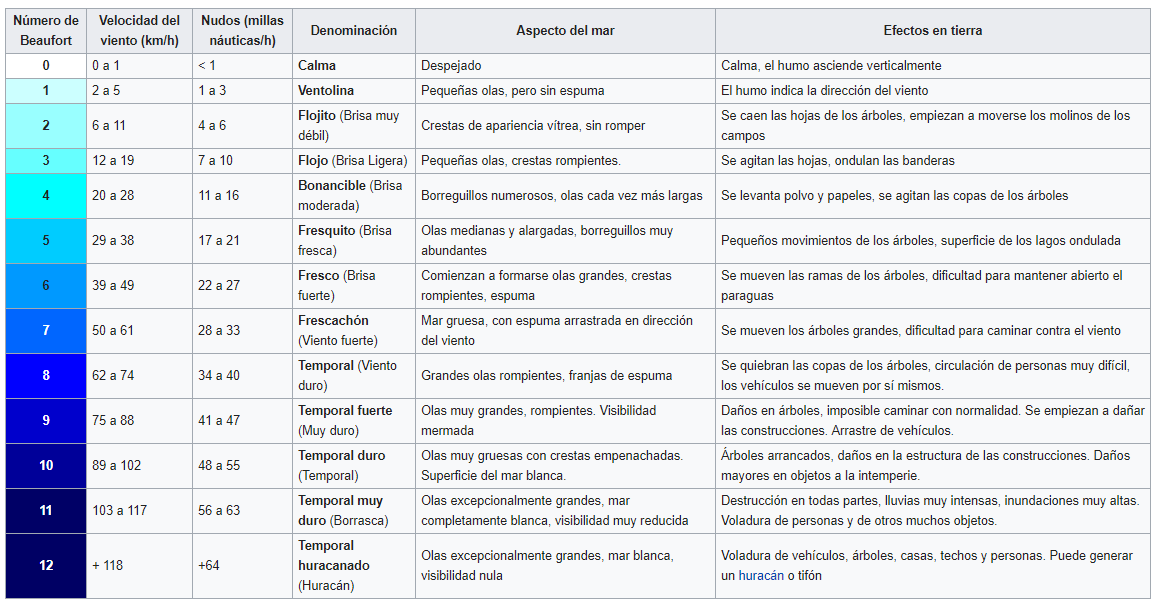
\includegraphics[scale=0.55]{escala_beaufort.png} 
  \caption{Escala Beaufort.}
\end{figure}

Entre una escala 3 y 7 serían los valores recomendados para practicar kitesurf sin riesgos,
 eso acota la velocidad del viento entre 12 y 61 Km/h, dato que nos será de utilidad
 en nuestra aplicación para hacernos una idea de los valores que recibiremos de
 un usuario que practique kitesurf. 

Practicar este deporte con vientos superiores, puede suponer para un deportista
 poco experimentado una situación de riesgo en la que nuestra aplicación puede
 tener mucha utilidad.
